% $Id: introduction.tex 87303 2016-02-08 13:44:29Z lafferty $
\clearpage
\newpage

\section{Appendix: Peaking background studies}
\label{app:background}

%{\it Give details on the \KL supression factor and on the \KLTpi}

The upper decay time acceptance (mainly the limited size of the VELO) causes the \KL reconstruction efficiency to be much lower than that of the \KS by about a factor of thousand ~\cite{KsmmANA}. We checked that a similar 
factor applies to our decay. Indeed, repeating the calculations of Sect.~6 in Ref.~\cite{KsmmANA} using our measured value of $\alpha_{\Kspizmm} = -110.9\pm 1.2 \; \rm ns^{-1}$ (see \figref{fig:lifetime}), we recovered an efficiency 
ratio factor of $\approx 2.2\times10^{-3}$.

\begin{figure} [htb!]
\begin{center}
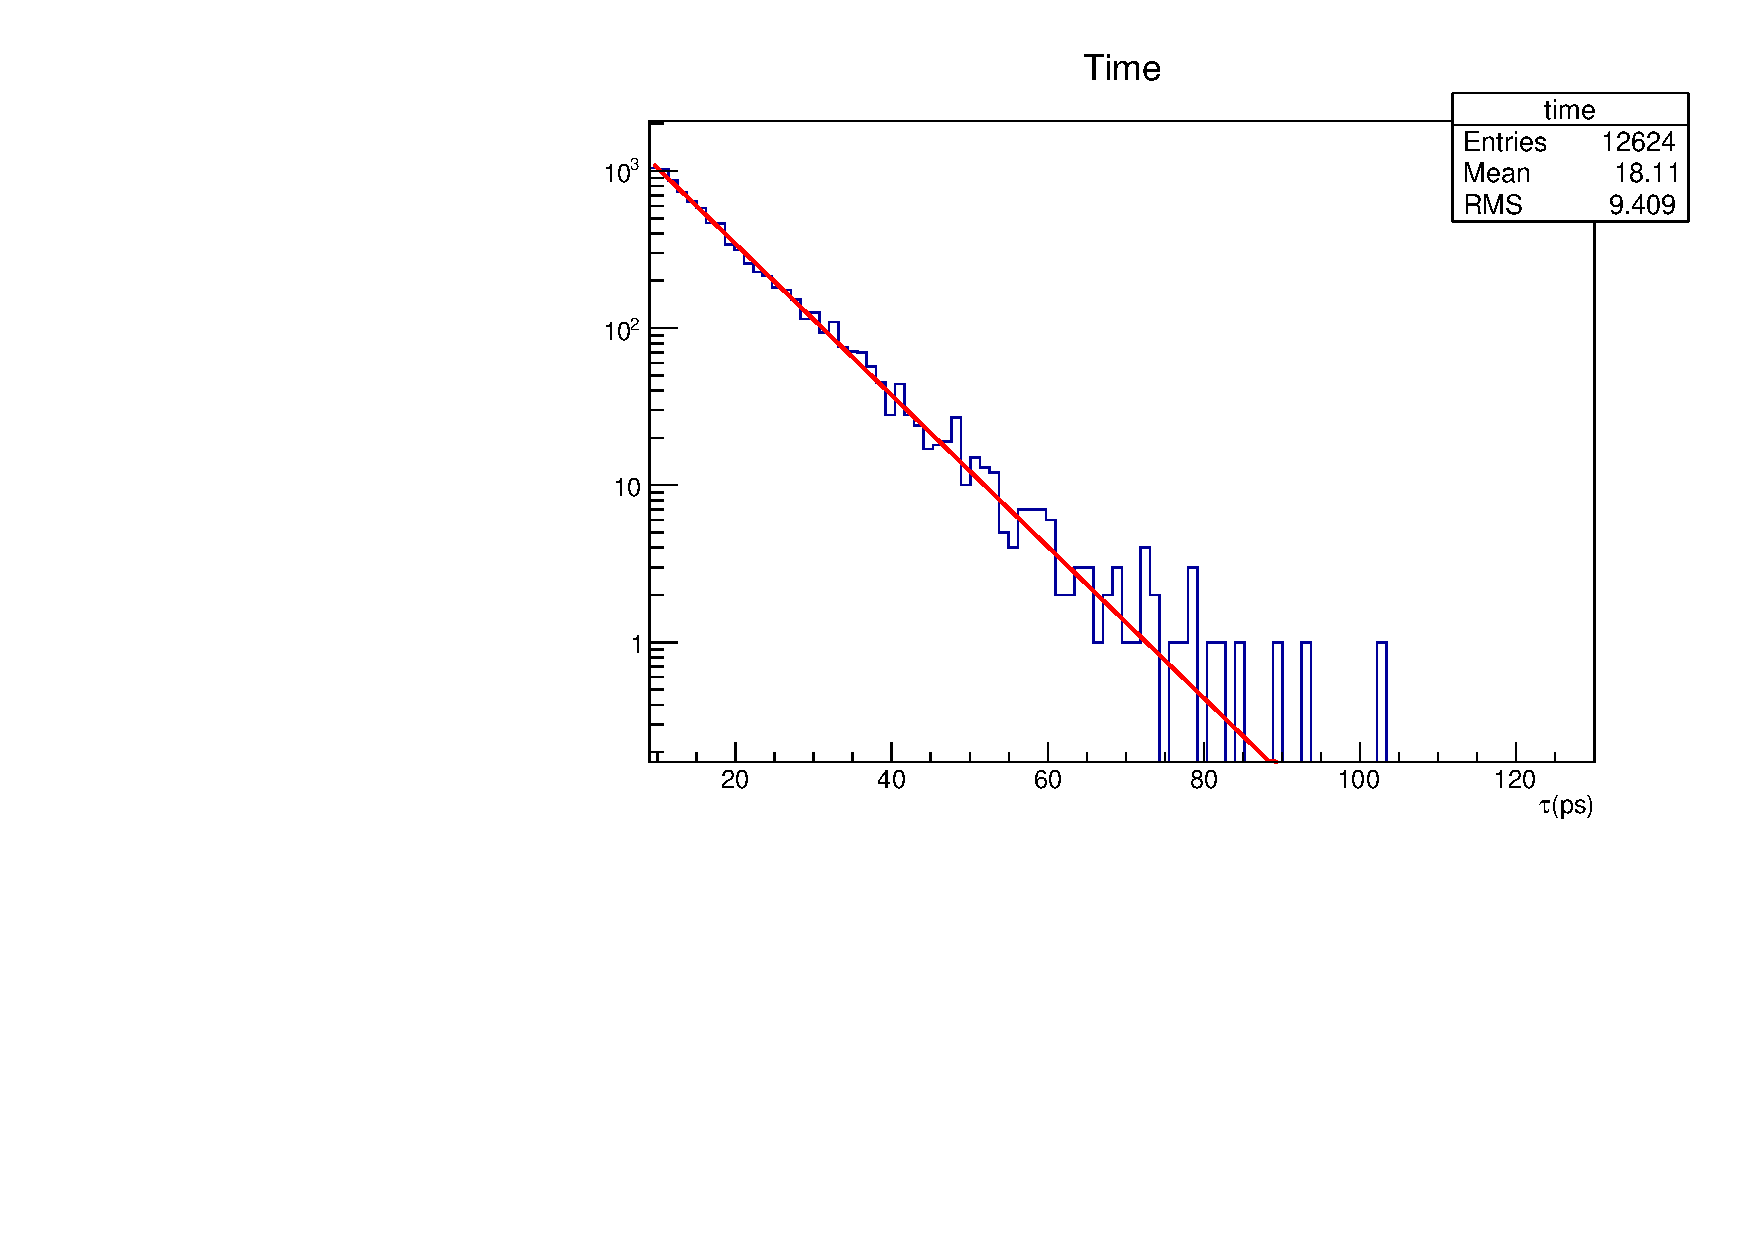
\includegraphics[scale=0.3]{figs/lifetime.pdf}
%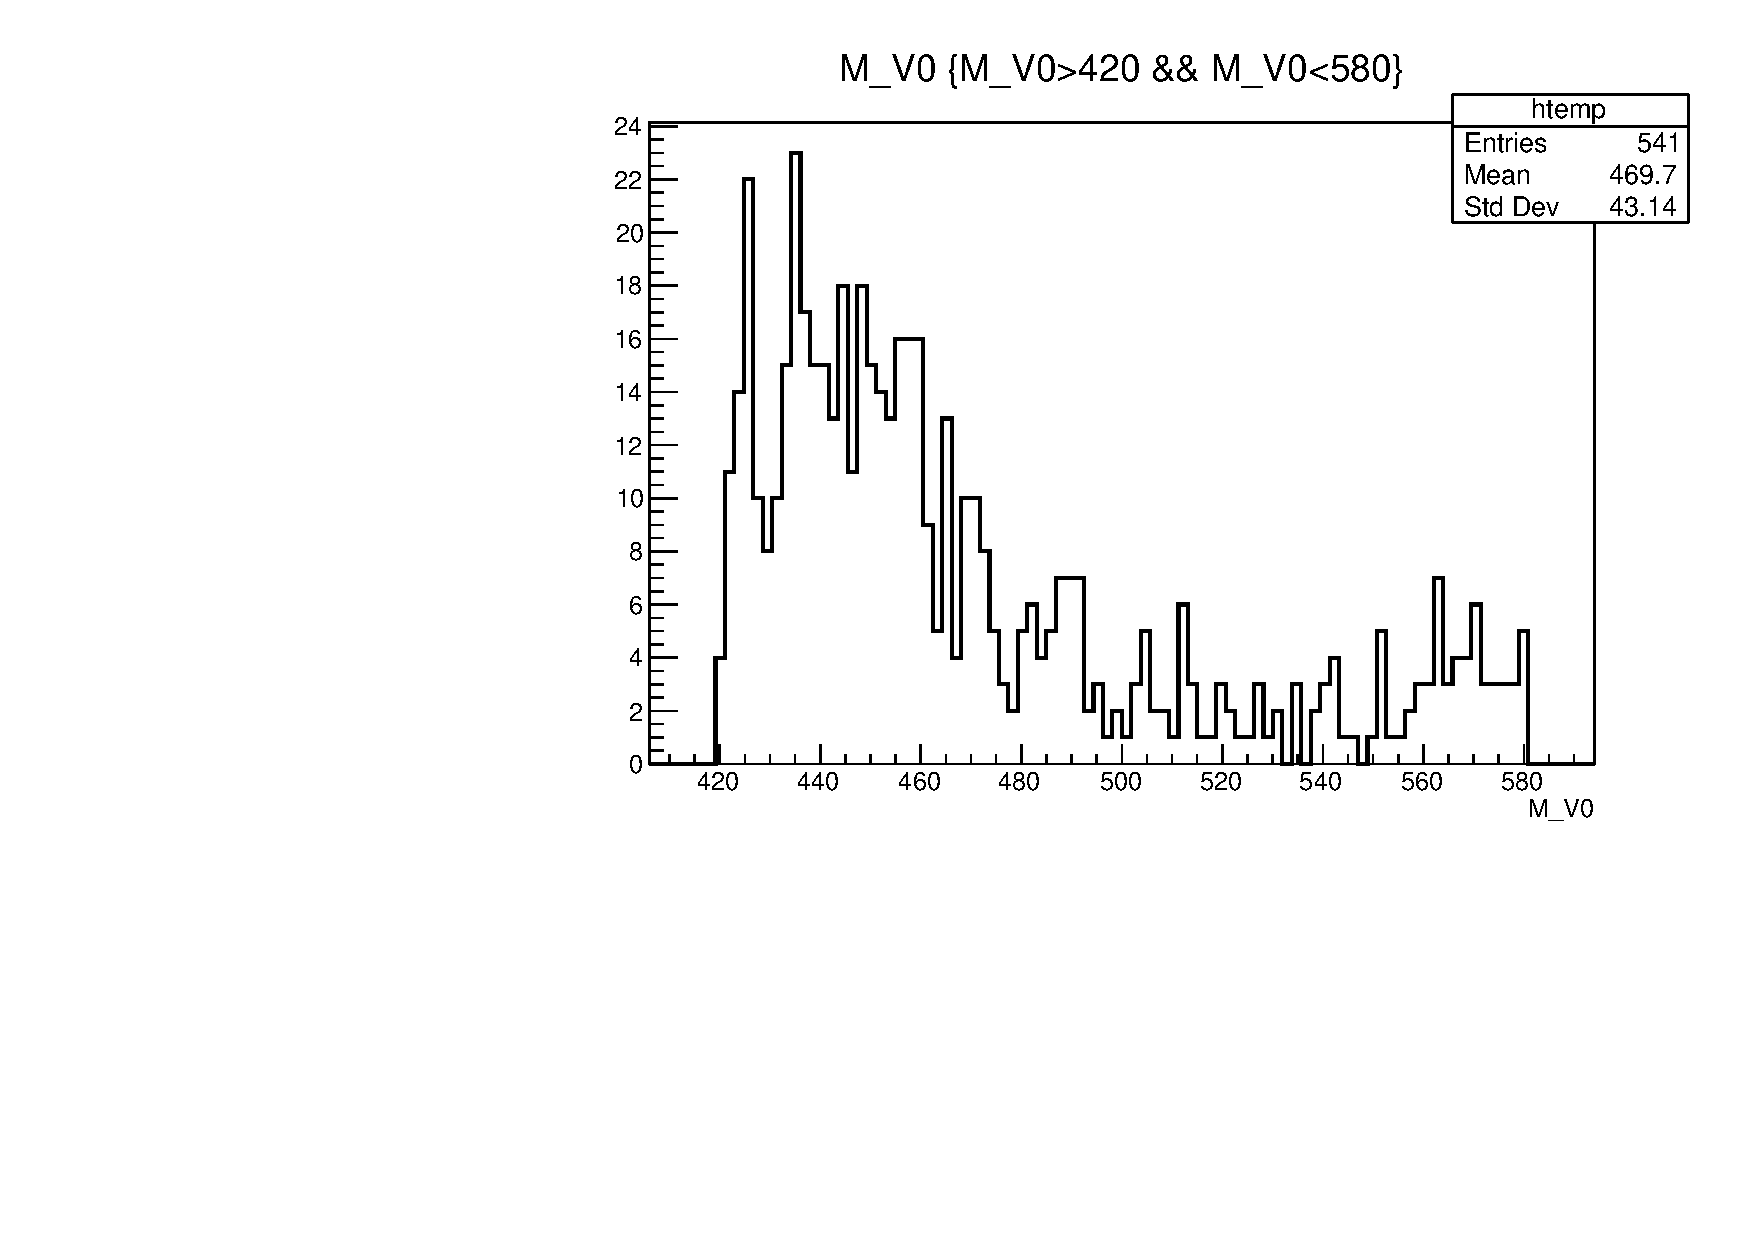
\includegraphics[scale=0.30]{figs/mK3pi_PARTIAL_wKsPiPi.pdf}
\caption{Lifetime distribution of selected \Kspizmm for $t>8.95\;\rm ps$. The red line shows an exponential fit, used to obtain $\alpha$~\cite{KsmmANA}. \label{fig:lifetime}}
\end{center}
\end{figure}


Samples of $K^0_S\rightarrow\pi^+\pi^-\pi^0$ corresponding to event type 34102408 were generated in order to study the \KLTpi  background.
The invariant mass distribution of the events stripped in a sample of $K^0_S\rightarrow\pi^+\pi^-\pi^0$ is shown in \figref{fig:KLTpi_wKspipi}. 
It can be seen as the right hand side bump (see also \figref{fig:mumuKspipi}) where we also included the \Kspipi from the underlying event and that also pass the selection. 
The Ismuon requirement was dropped from the stripping to increase the statistics. We find 254 \Kspipi out of 735 candidates. Taking into account the suppresion factor for \KL to \KS ($\sim2\times10^{-3}$), 
the MC generation efficiency ($\approx 0.36$) and the fact that the $3\pi$ decays is forced, we expect a ratio of $\sim2\times10^{-4}$ \KLTpi per \Kspipi decay in our PARTIAL background. 
A stripping 21 (i.e, FULL) filtered \KSTpi sample is also available. In that case we find about $50\%$  of the events actually come from the forced decay. Again, taking into account the \KL to \KS supression factor, 
we find that this background is small compared to other sources. The BDT and mass distributions of the 18 events of the filtered sample which also pass the selection cuts applied prior to BDT training is shown in 
\figref{fig:KLTpi_BDT}. No events are in the BDT region used for the fit, and the effective luminosity of the sample is insufficient to derive a meaningful quantitative upper limit on the number of \KLTpi events expected 
in the data. Finally, in order to asess the possible impact on the sensitivity, we add to the fit a Landau component with parameters fixed to those obtained from simulation at the stripping filtered level (we lack 
statistics to do it after all cuts and per BDT bin), as shown in \figref{fig:Landau}. The fit to data is shown in \figref{fig:fitK3pi}. The expected sensitivity for 50 fb$^{-1}$ including this component is 
$\pm5.3\times10^{-9}$, very similar to the one obtained when this component is ignored, $5.5\times10^{-9}$. The size of the Landau component is consistent with zero at one sigma in all BDT bins.


   
To study the contribution of a background due to three-pion final state decays, such as $\eta\to\pi^+\pi^-\pi^0$, the invariant $K^{0}$ mass is reconstructed using the pion mass hypothesis
for the muons. The corresponding distributions are shown in \figref{fig:eta_bkg}. No peaking structures in the signal region are to be seen.
   
\begin{figure} [htb!]
\begin{center}
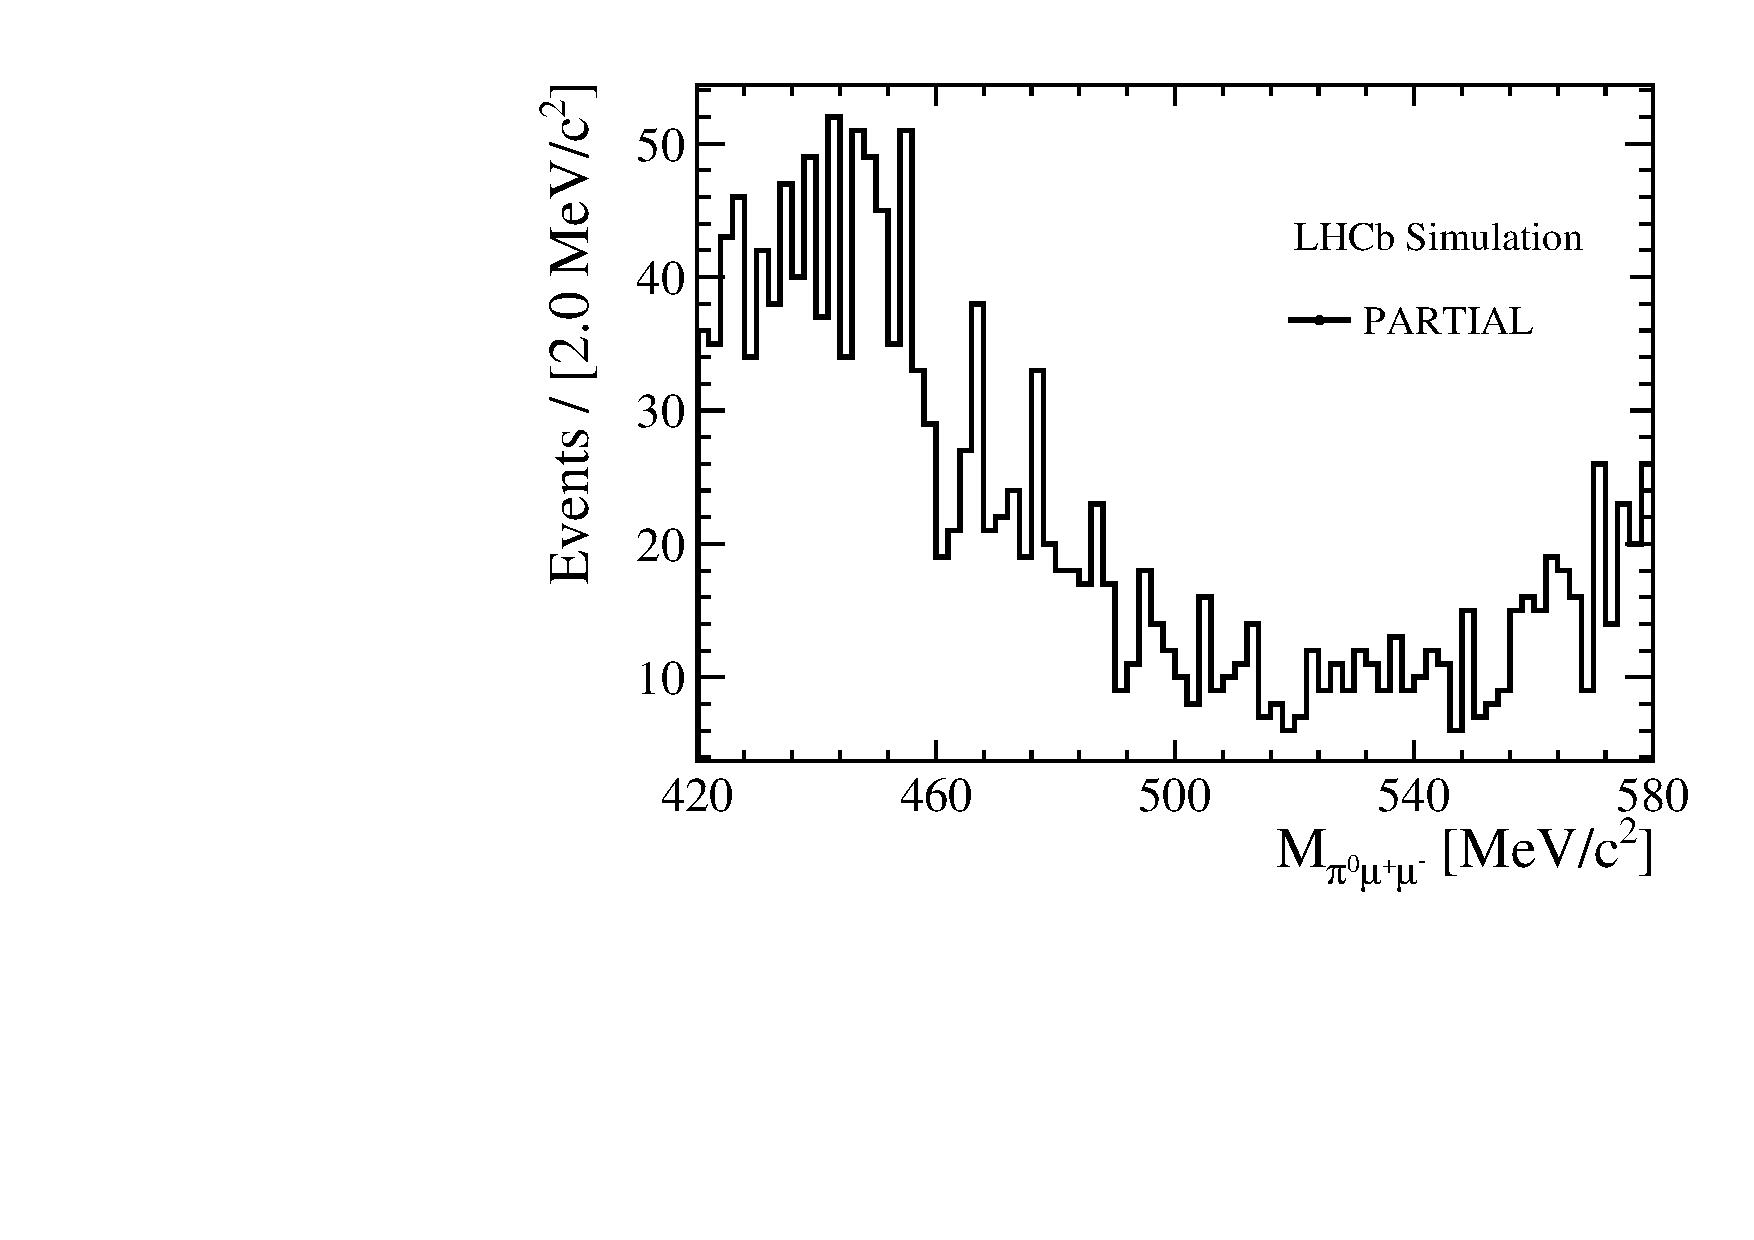
\includegraphics[scale=0.60]{figs/M_V0_K3pi_Kspipi.pdf}%{figs/mK3pi_PARTIAL_wKsPiPi.pdf}
%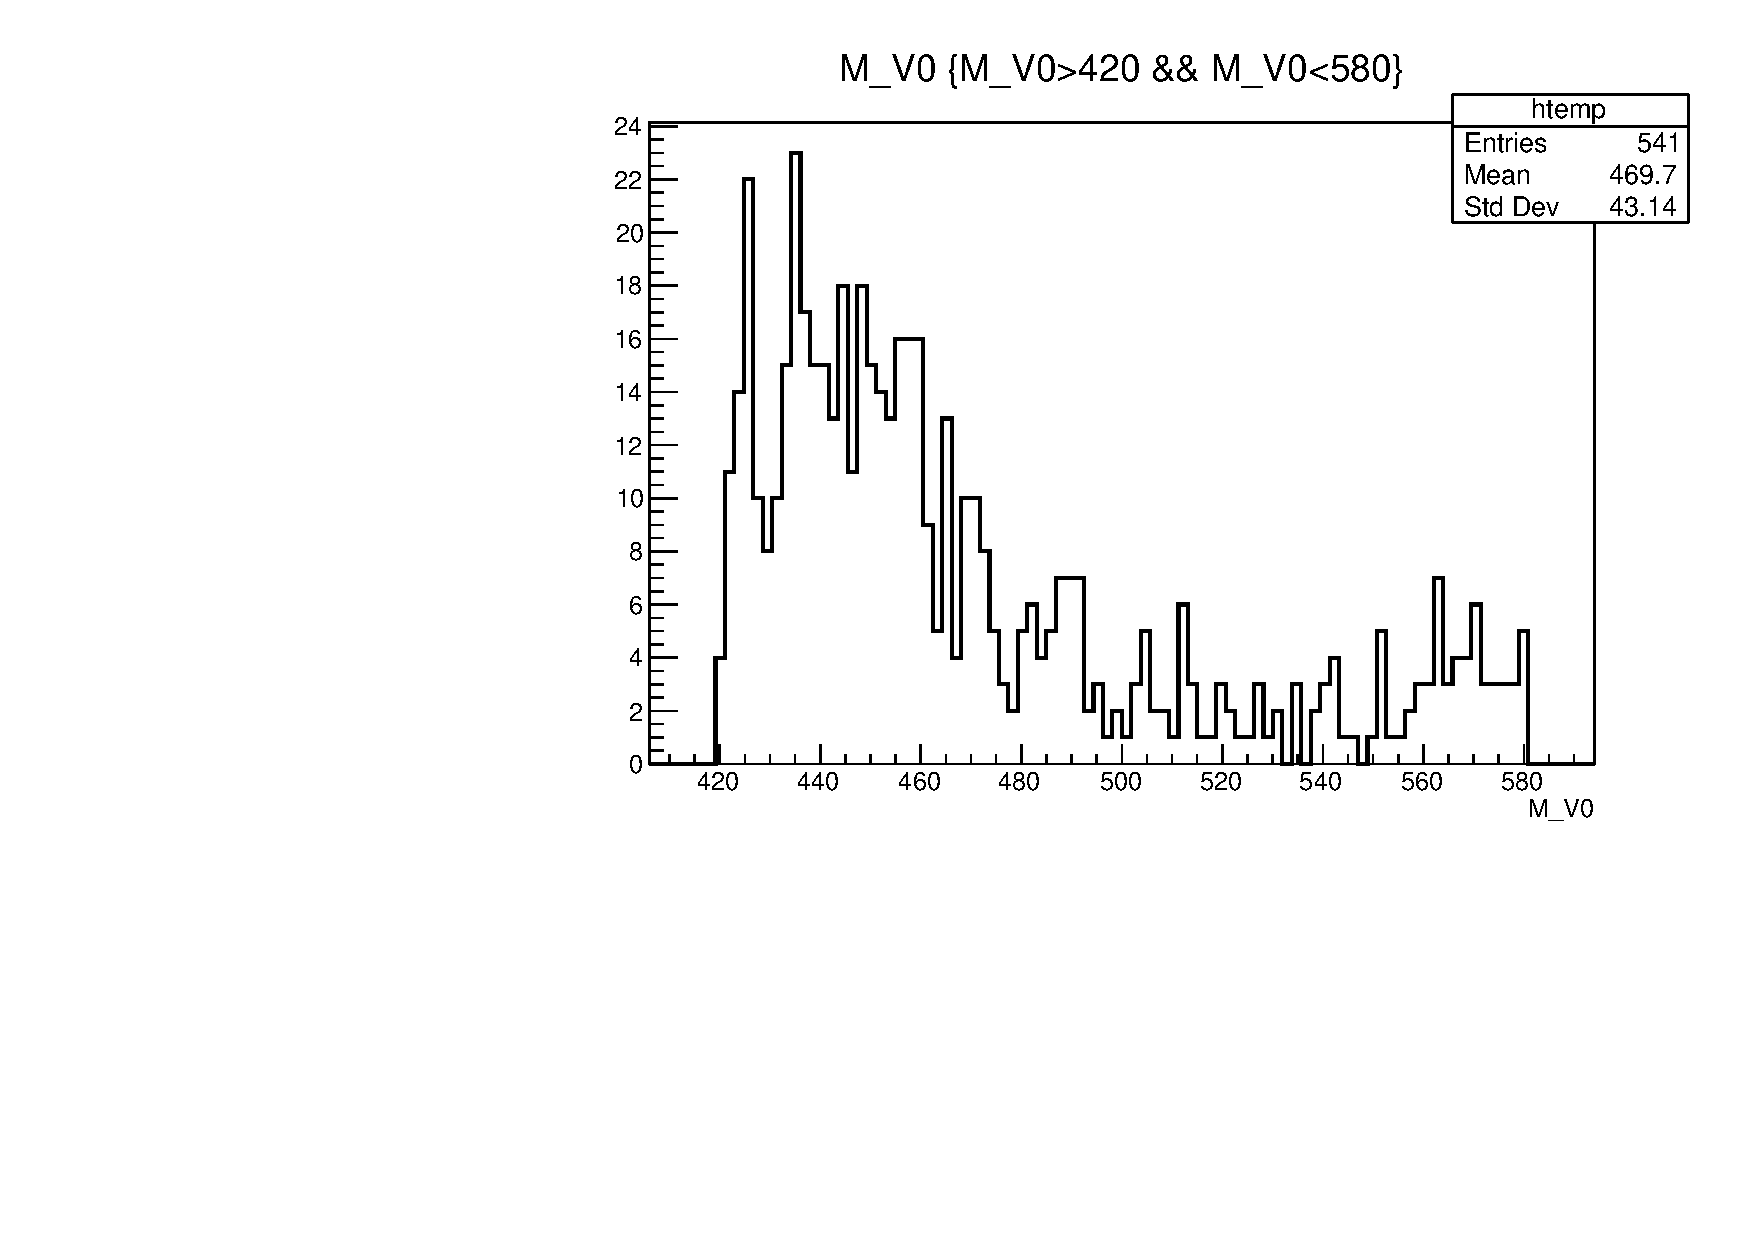
\includegraphics[scale=0.30]{figs/mK3pi_PARTIAL_wKsPiPi.pdf}
\caption{Invariant mass distribution of simulated $K^0\rightarrow\pi^+\pi^-\pi^0$ decays selected in the PARTIAL category including also the \Kspipi decays that got selected from the underlying event, 
which can be seen as the right hand side bump. \label{fig:KLTpi_wKspipi}}
\end{center}
\end{figure}
   
\begin{figure} [htb!]
\begin{center}
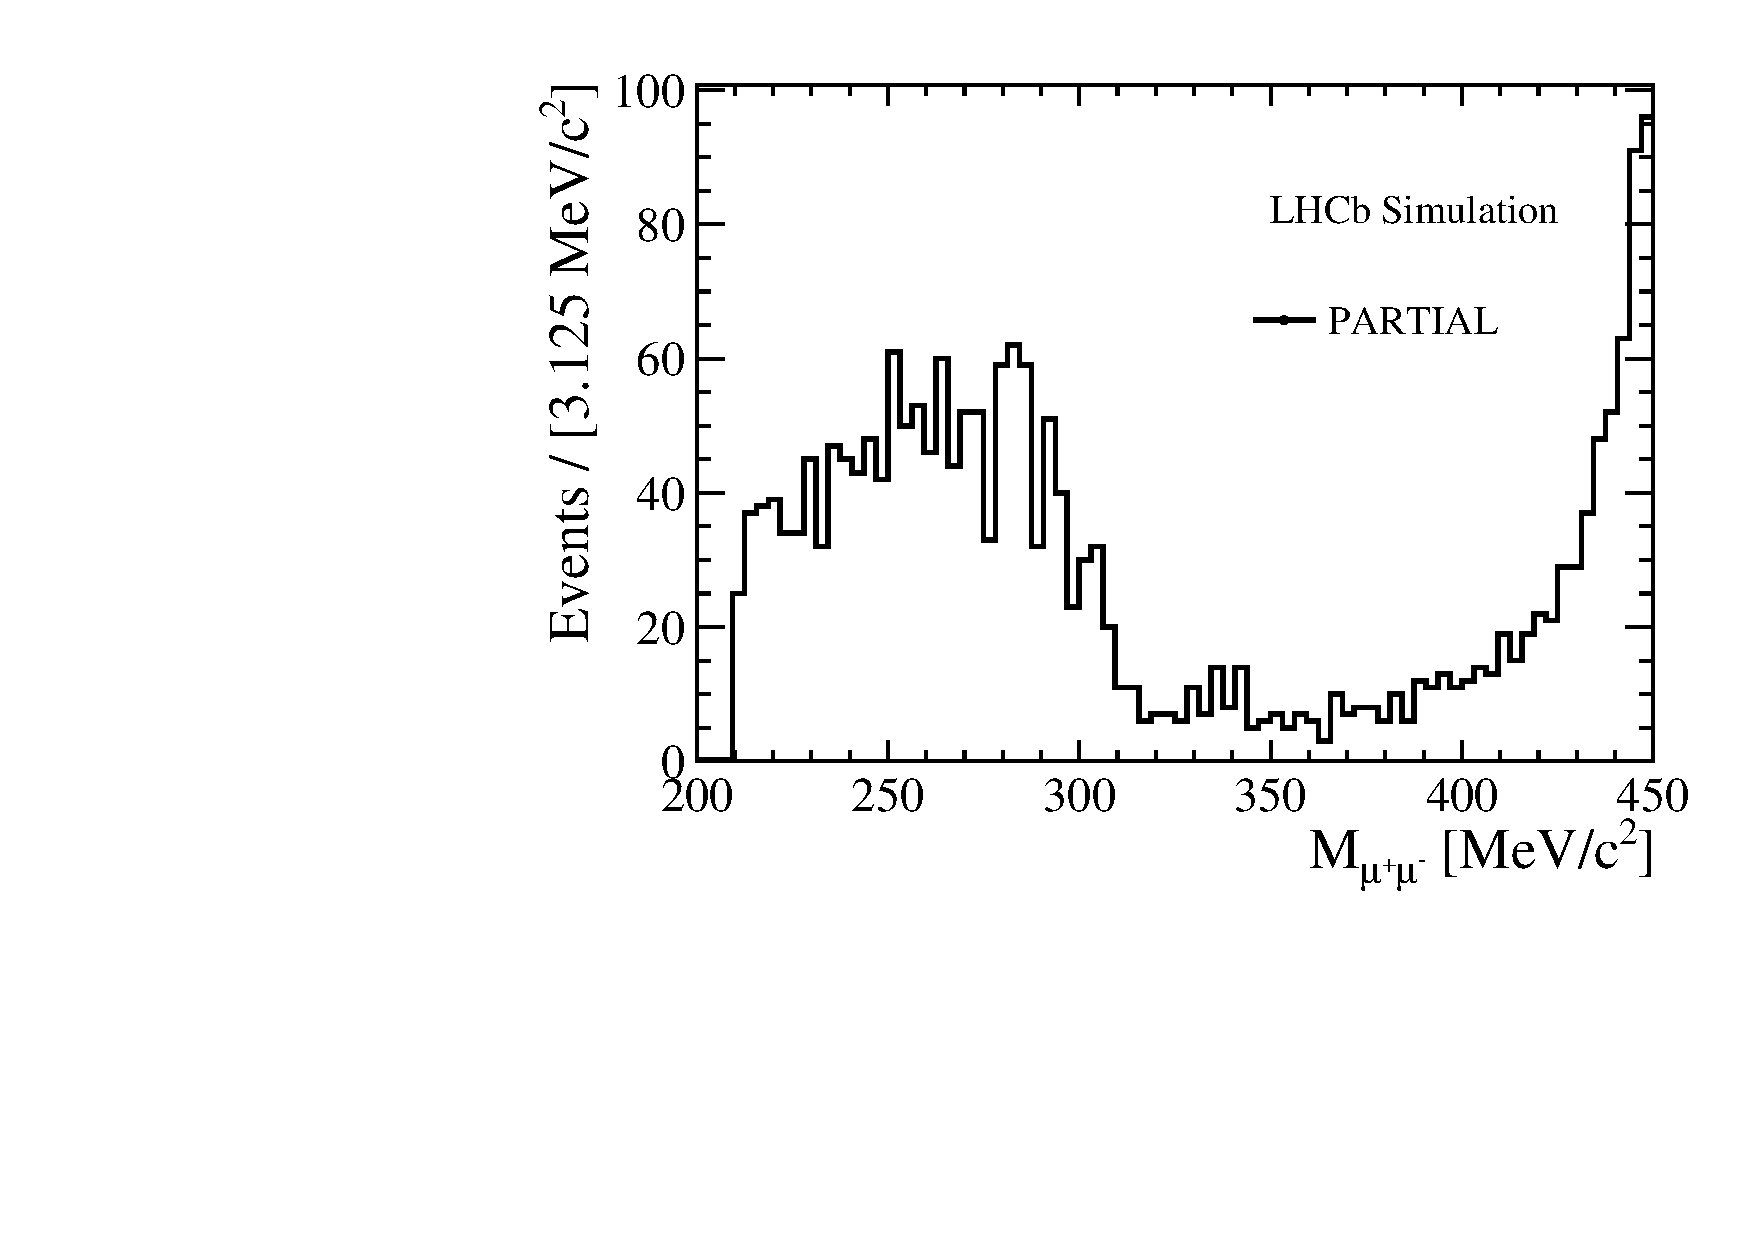
\includegraphics[scale=0.60]{figs/M_mumu_K3pi_Kspipi.pdf}%{figs/mumu_mass.pdf}
%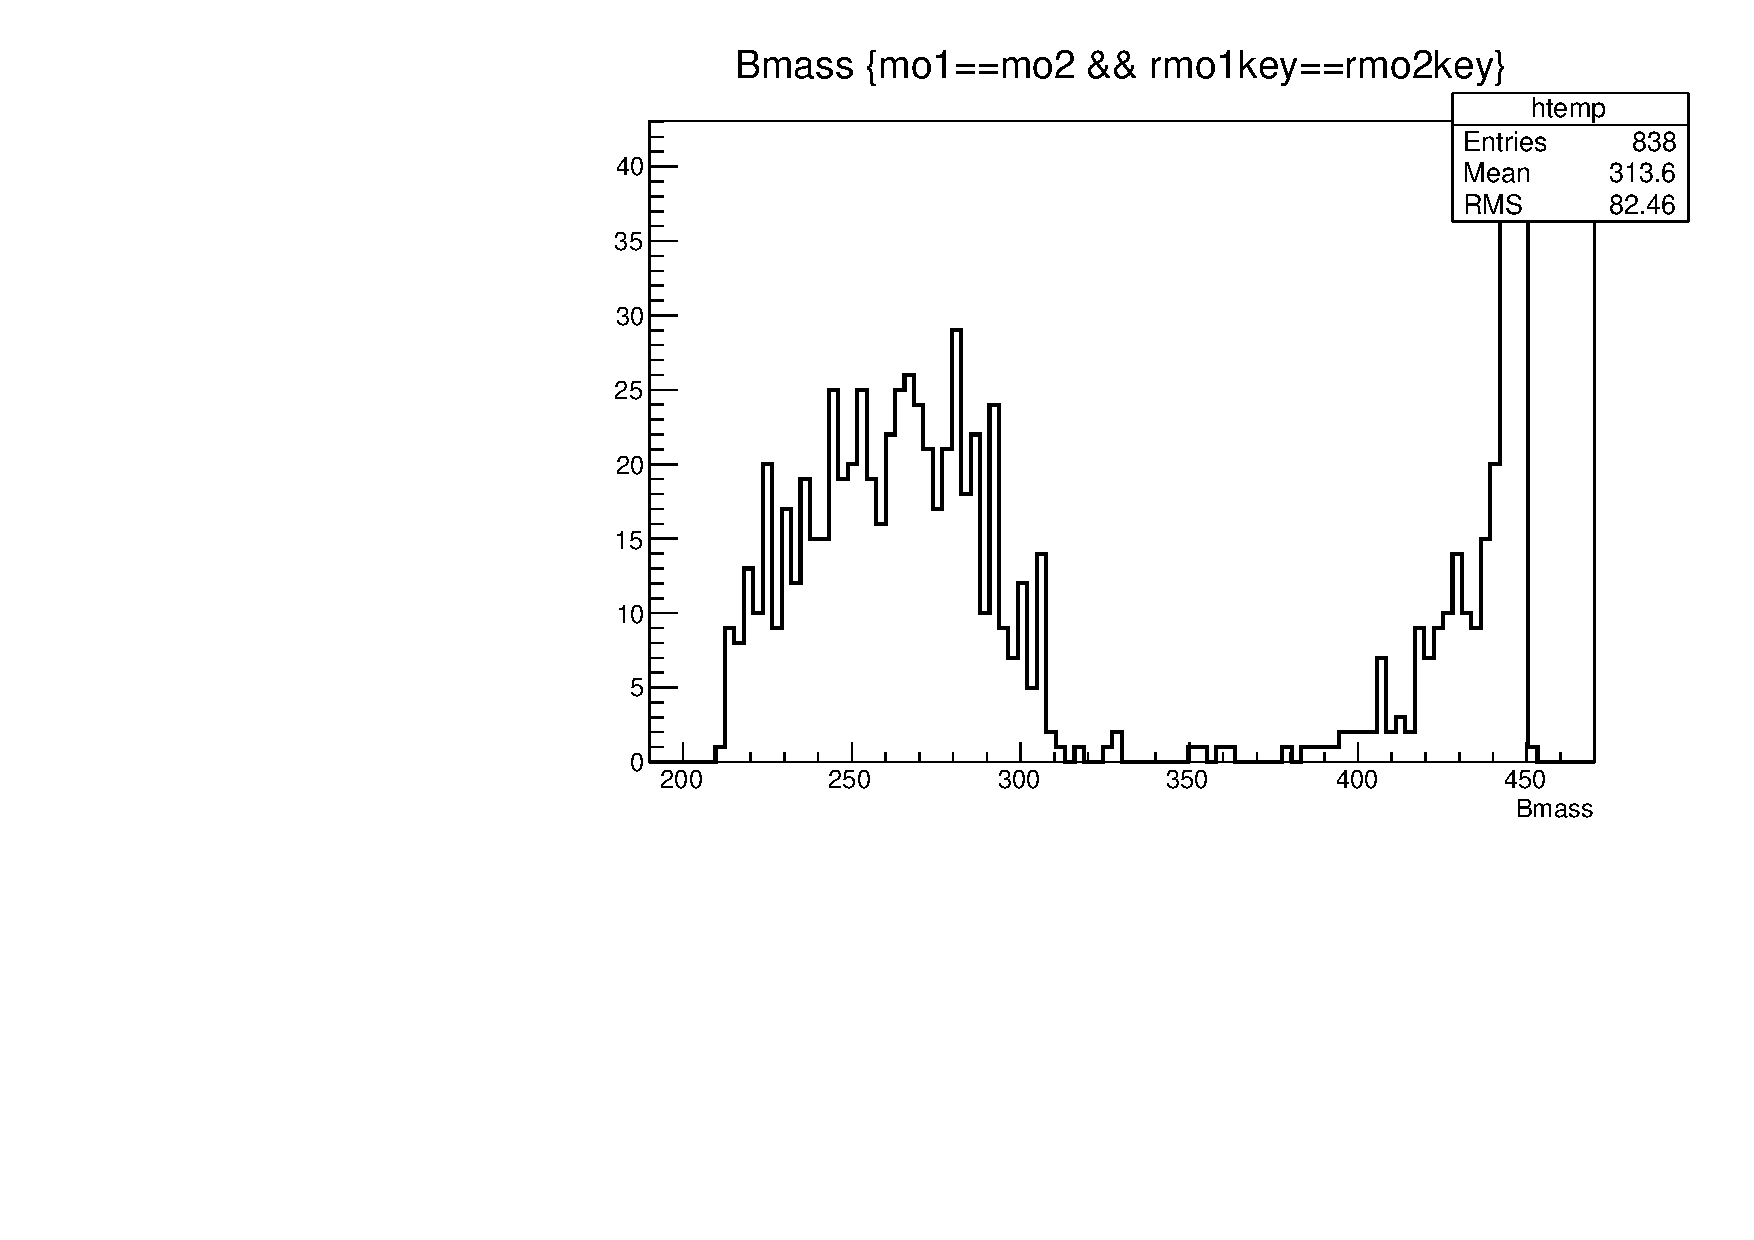
\includegraphics[scale=0.30]{figs/mumu_mass.pdf}
\caption{Invariant mass distribution of dimuon candidates in simulated $K^0\rightarrow\pi^+\pi^-\pi^0$ decays selected in the PARTIAL category, and including also the \Kspipi that got selected from the underlying event. 
\label{fig:mumuKspipi}}
\end{center}
\end{figure}

\begin{figure} [htb!]
\begin{center}
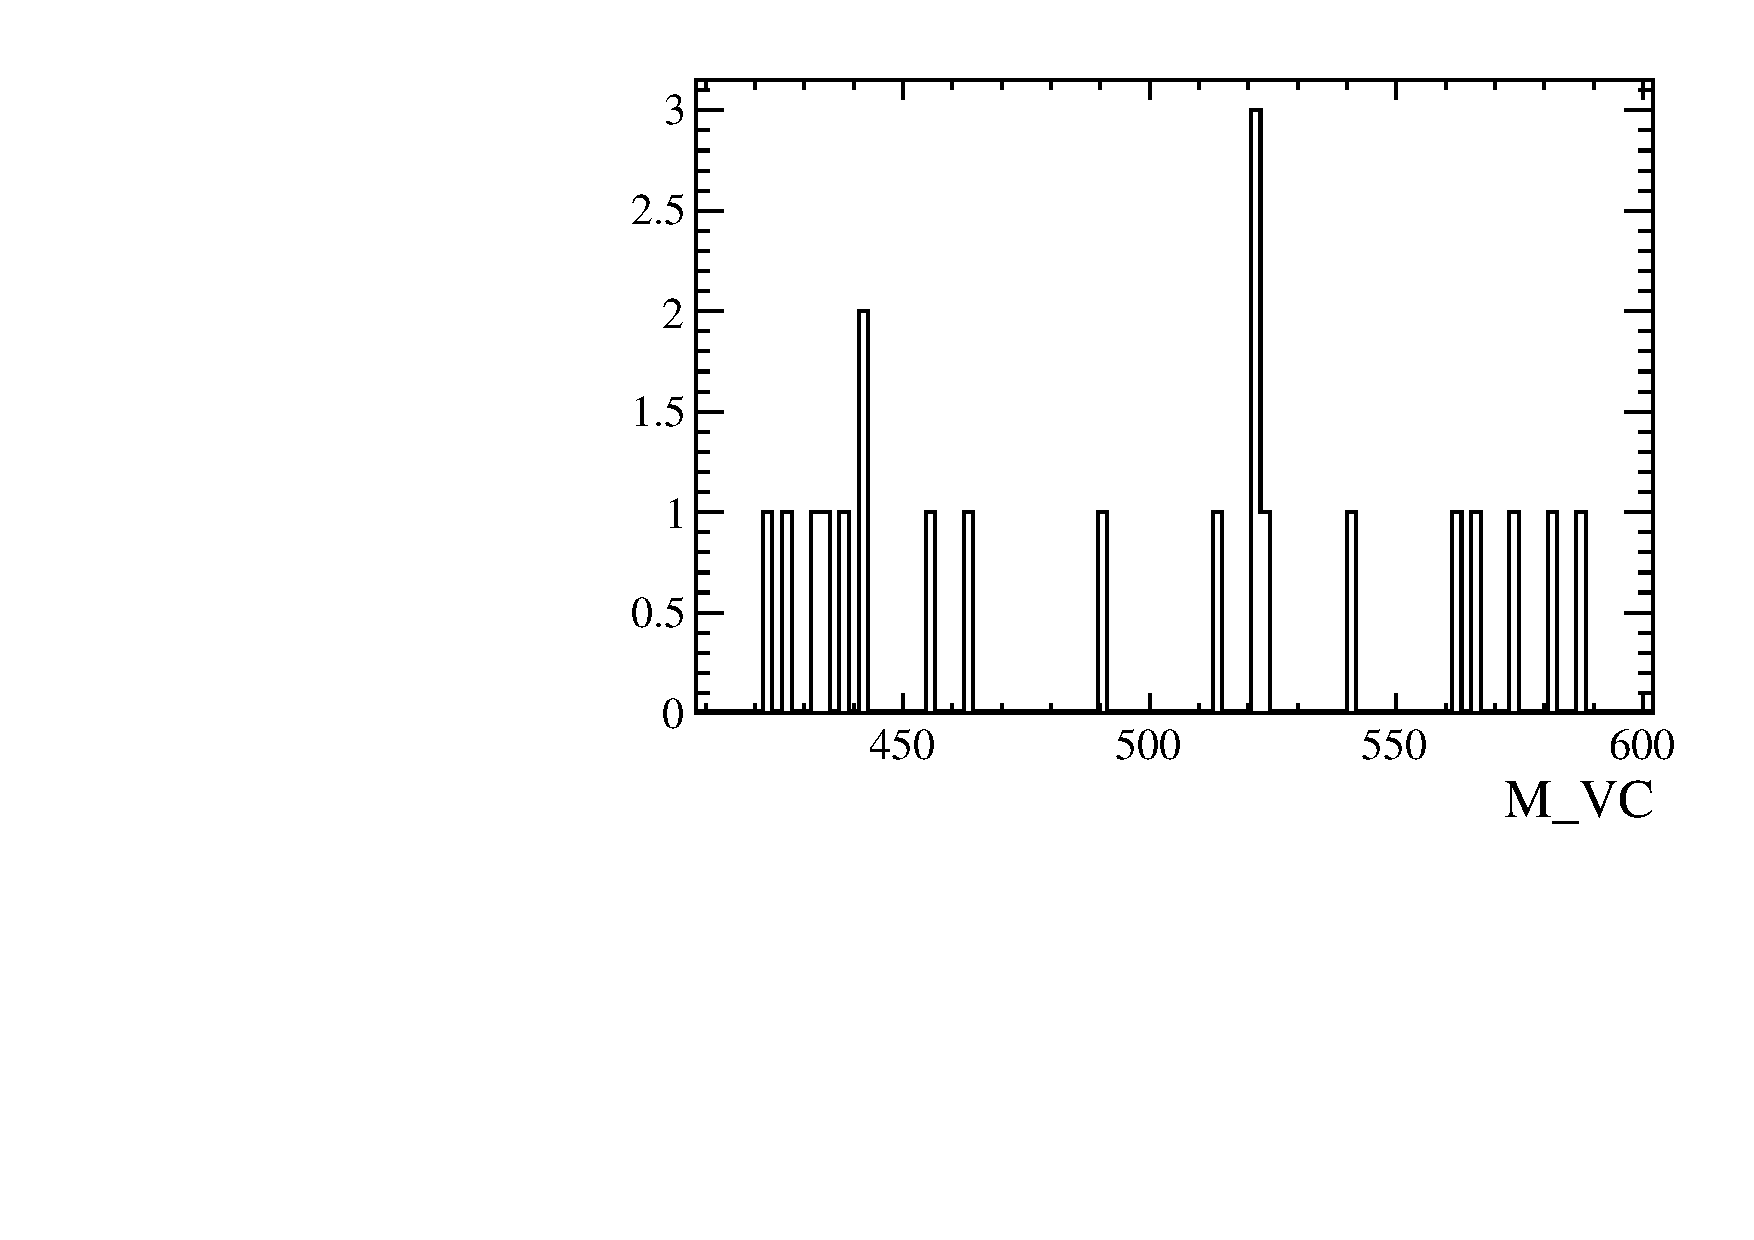
\includegraphics[scale=0.3]{figs/filtered_mass_BDTintegrated.pdf}
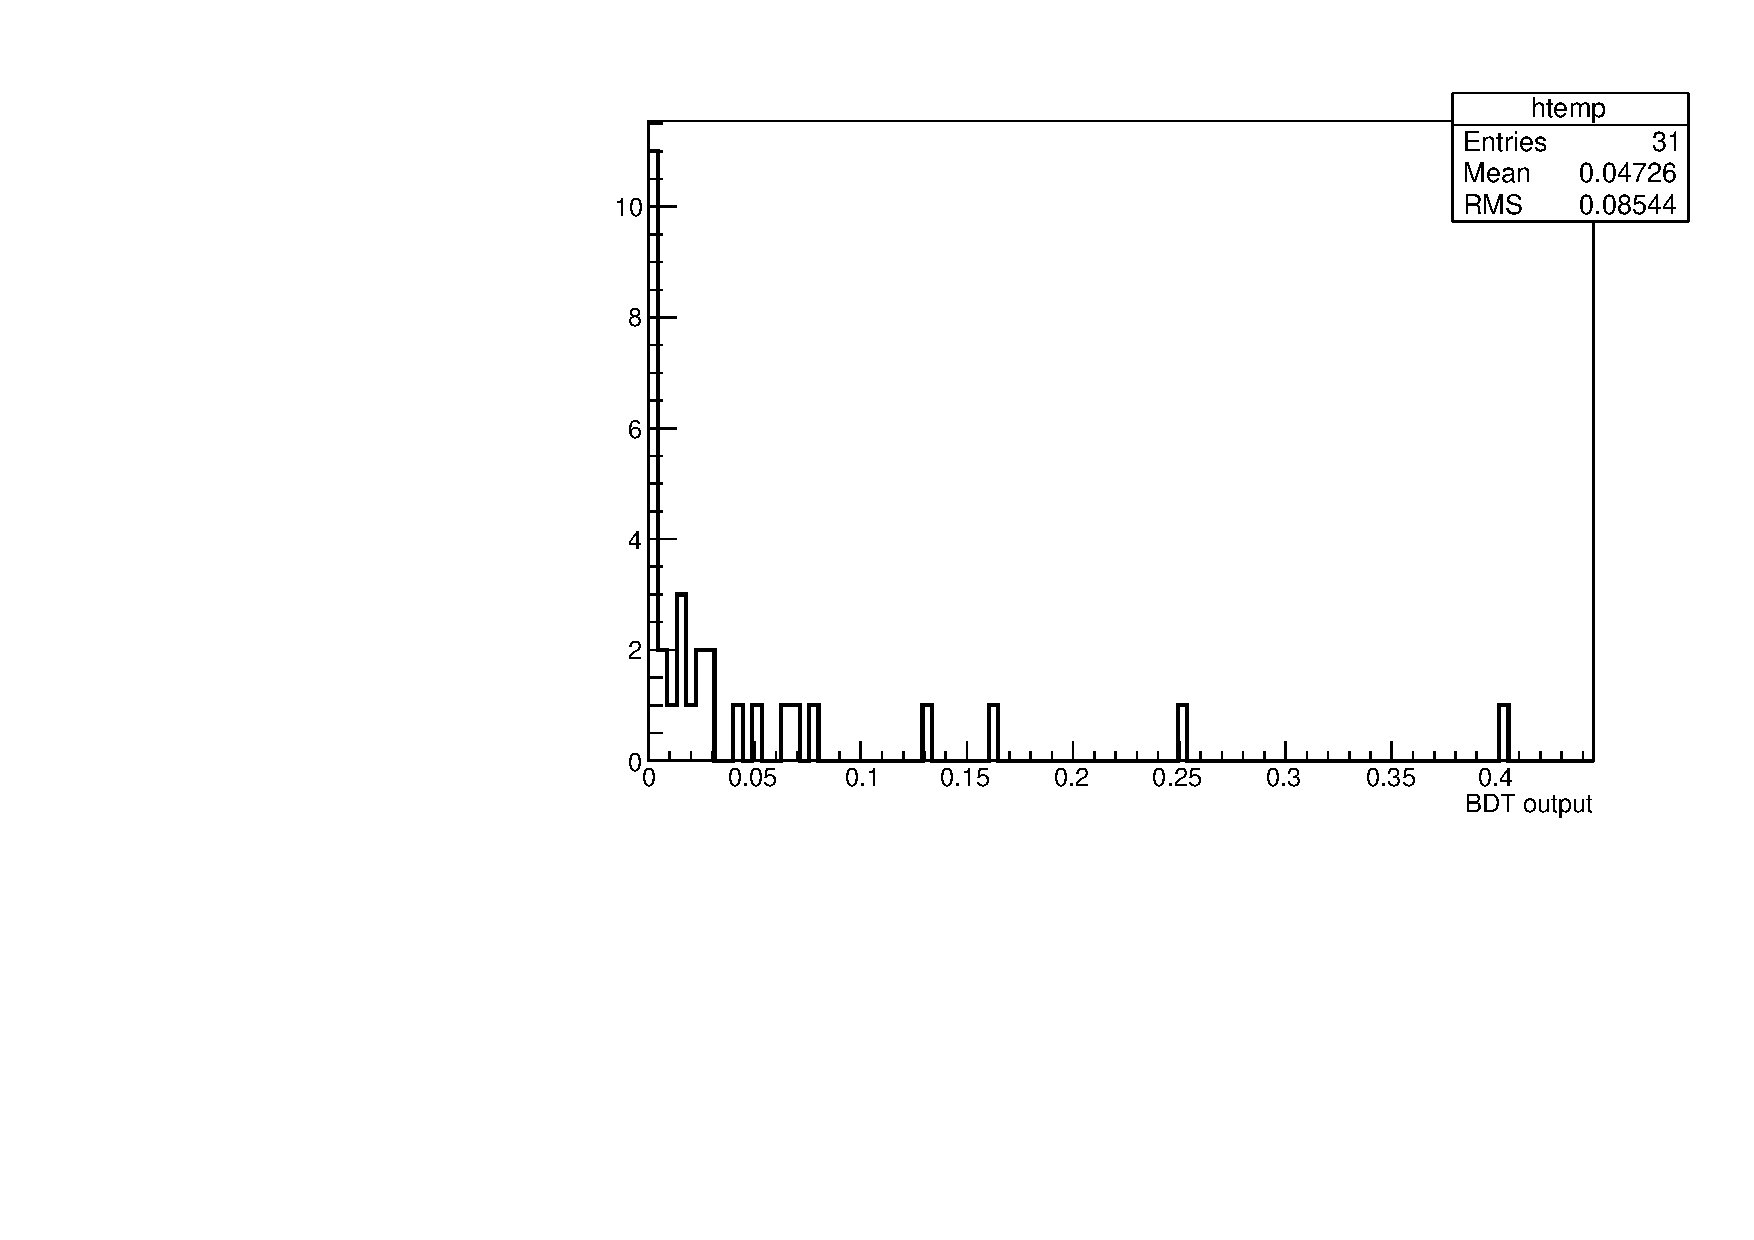
\includegraphics[scale=0.30]{figs/K3pi_BDT.pdf}
\caption{Mass and BDT distribution of the \KSTpi simulated FULL candidates.\label{fig:KLTpi_BDT}}
\end{center}
\end{figure}
\begin{figure} [htb!]
\begin{center}
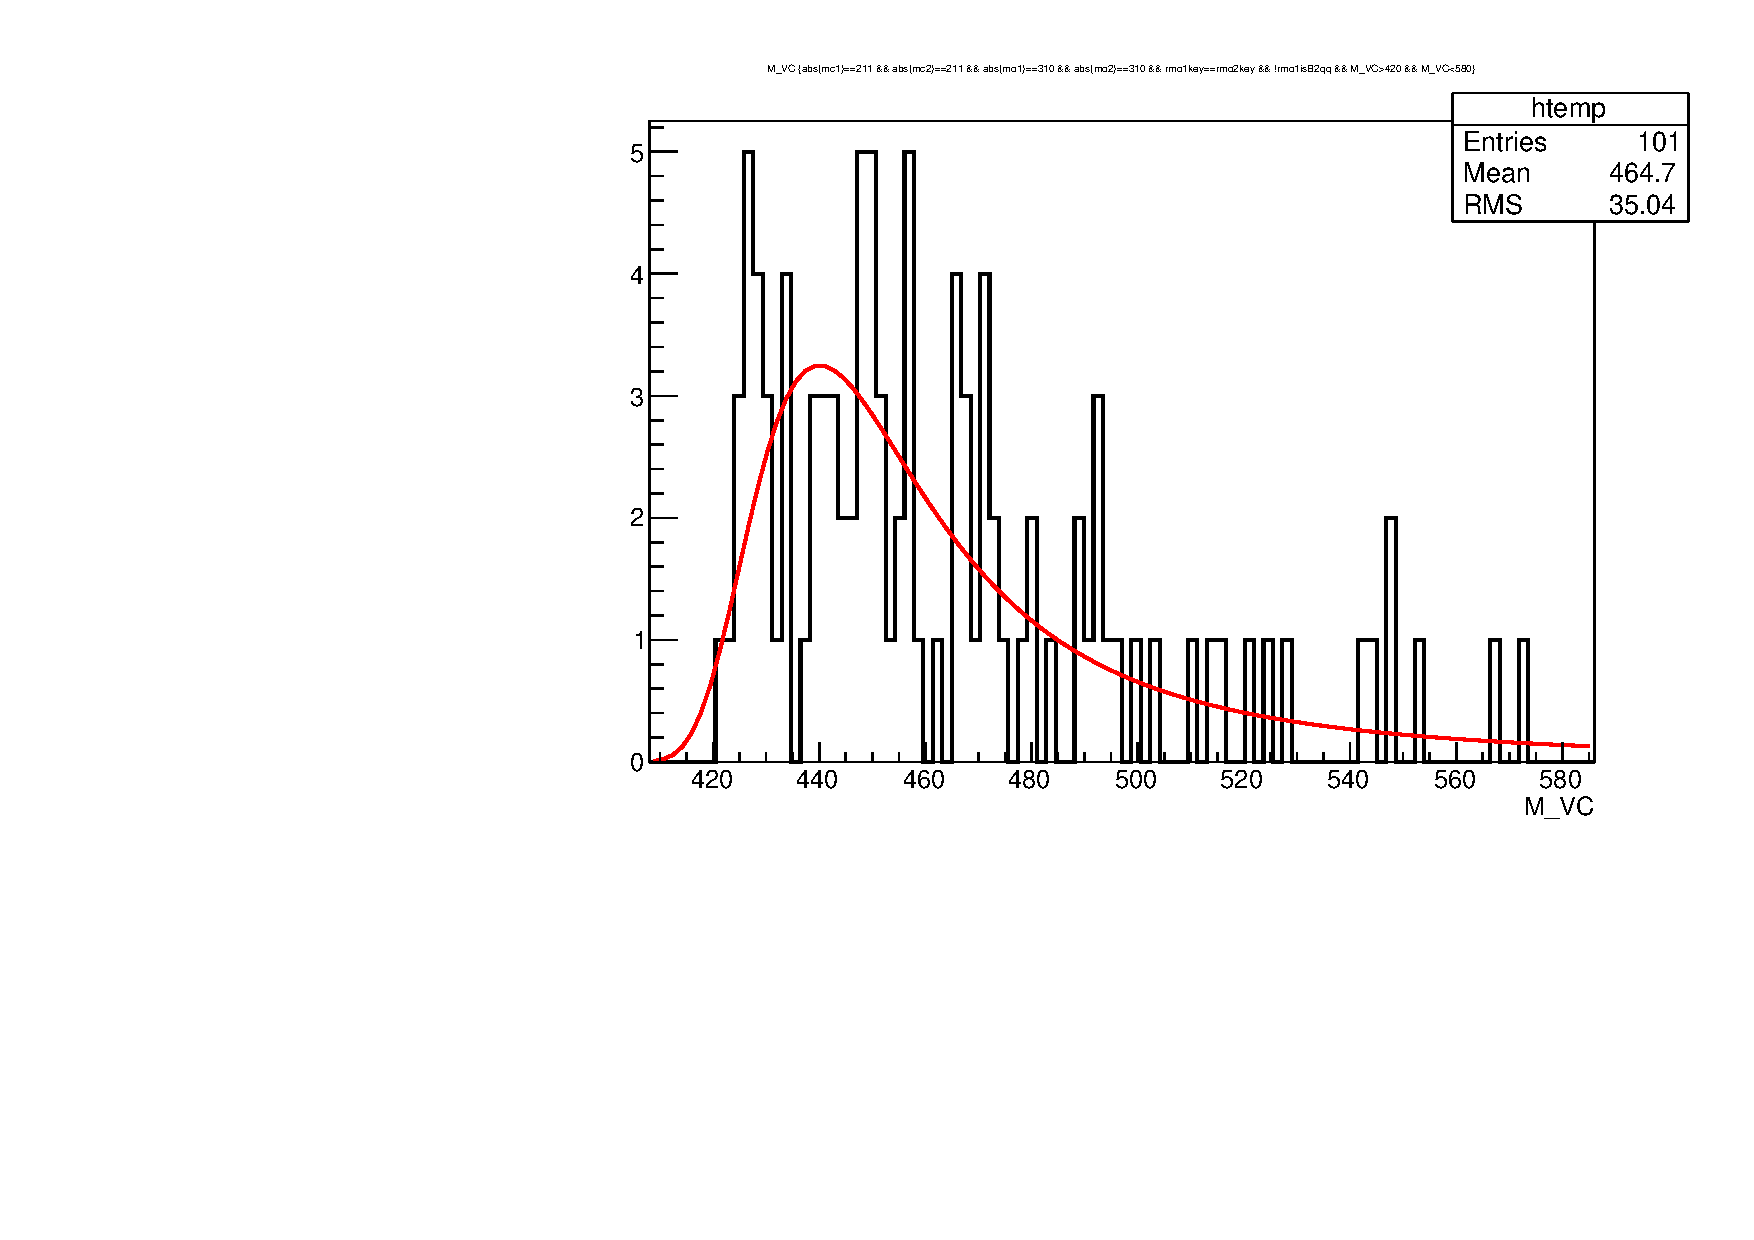
\includegraphics[scale=0.6]{figs/landau.pdf}
\caption{Mass of \KSTpi after stripping FULL, and fit to a Landau \pdf. \label{fig:Landau}}
\end{center}
\end{figure}

\begin{figure} [htb!]
\begin{center}
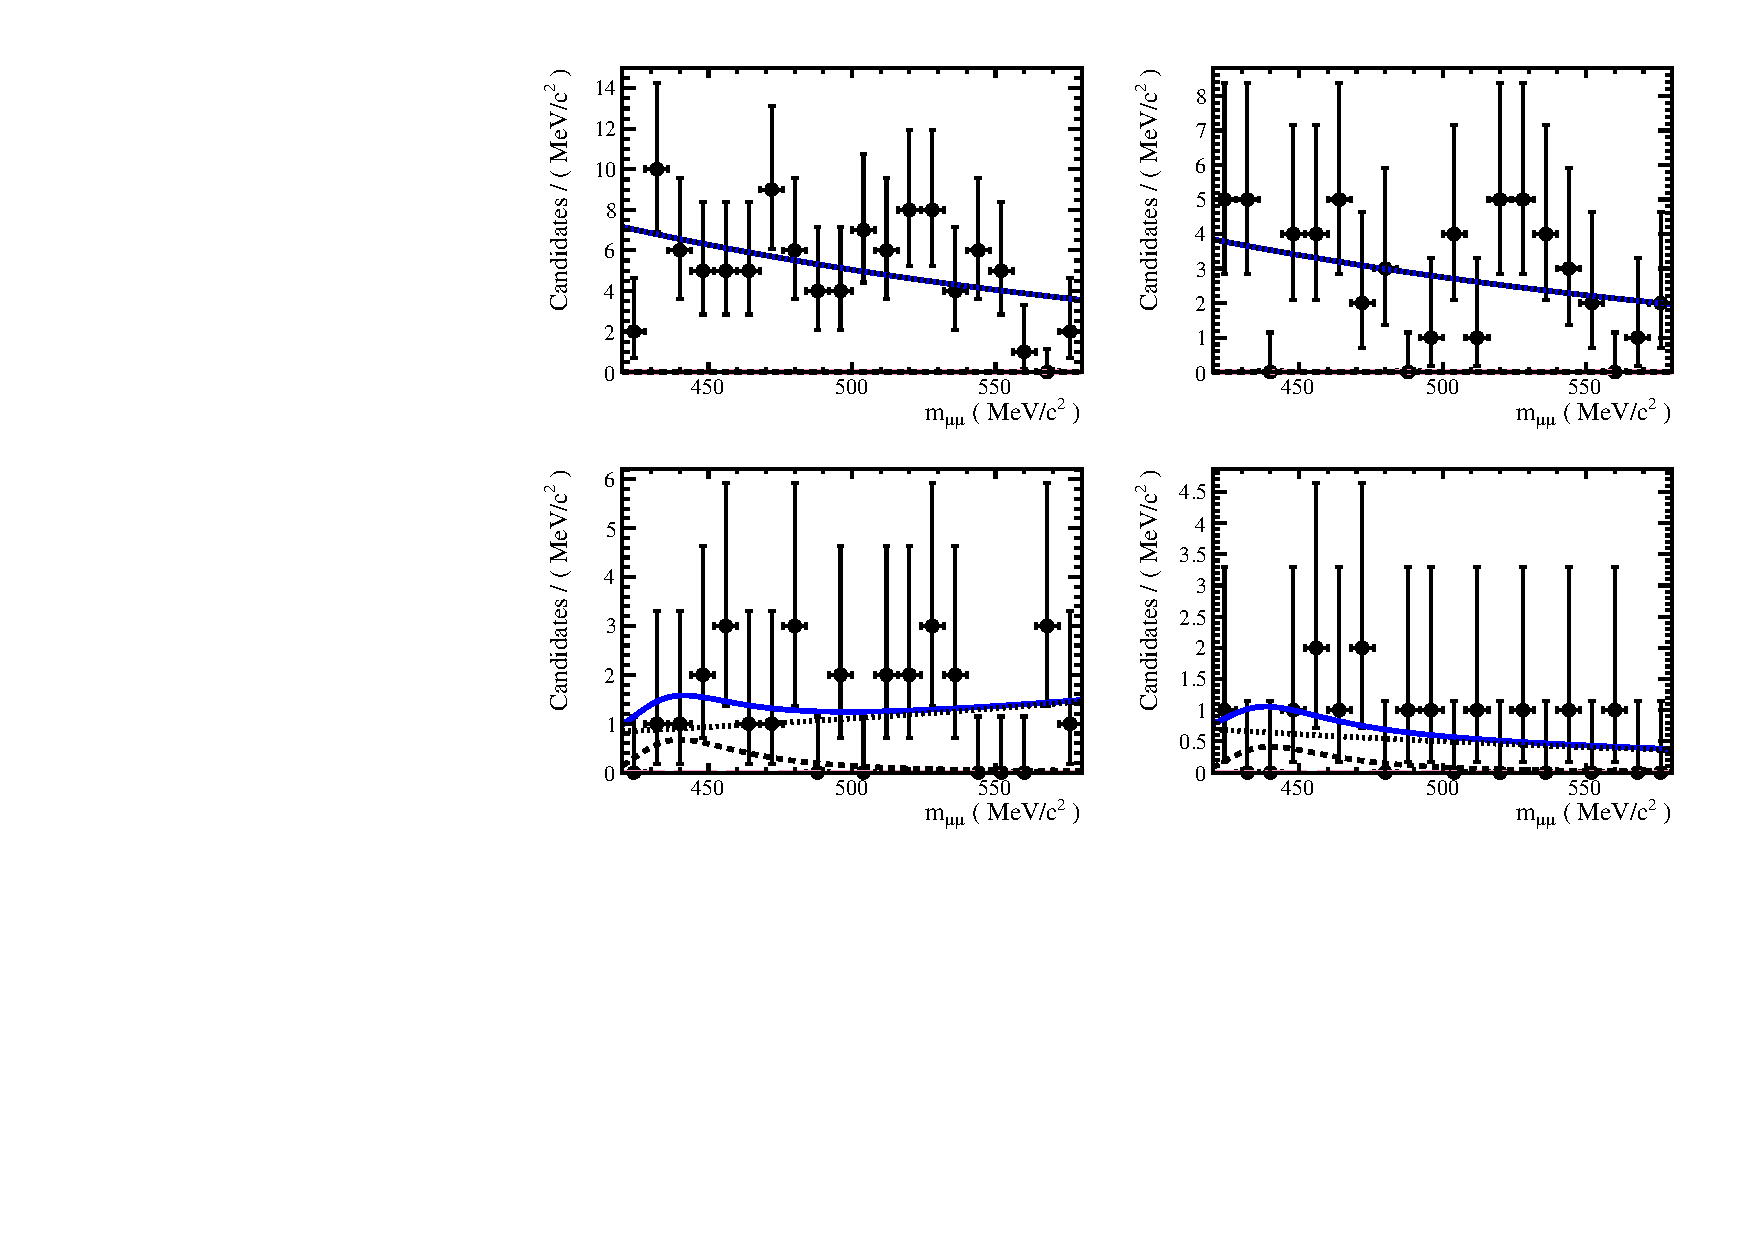
\includegraphics[scale=0.5]{figs/fit_wK3pi.pdf}
%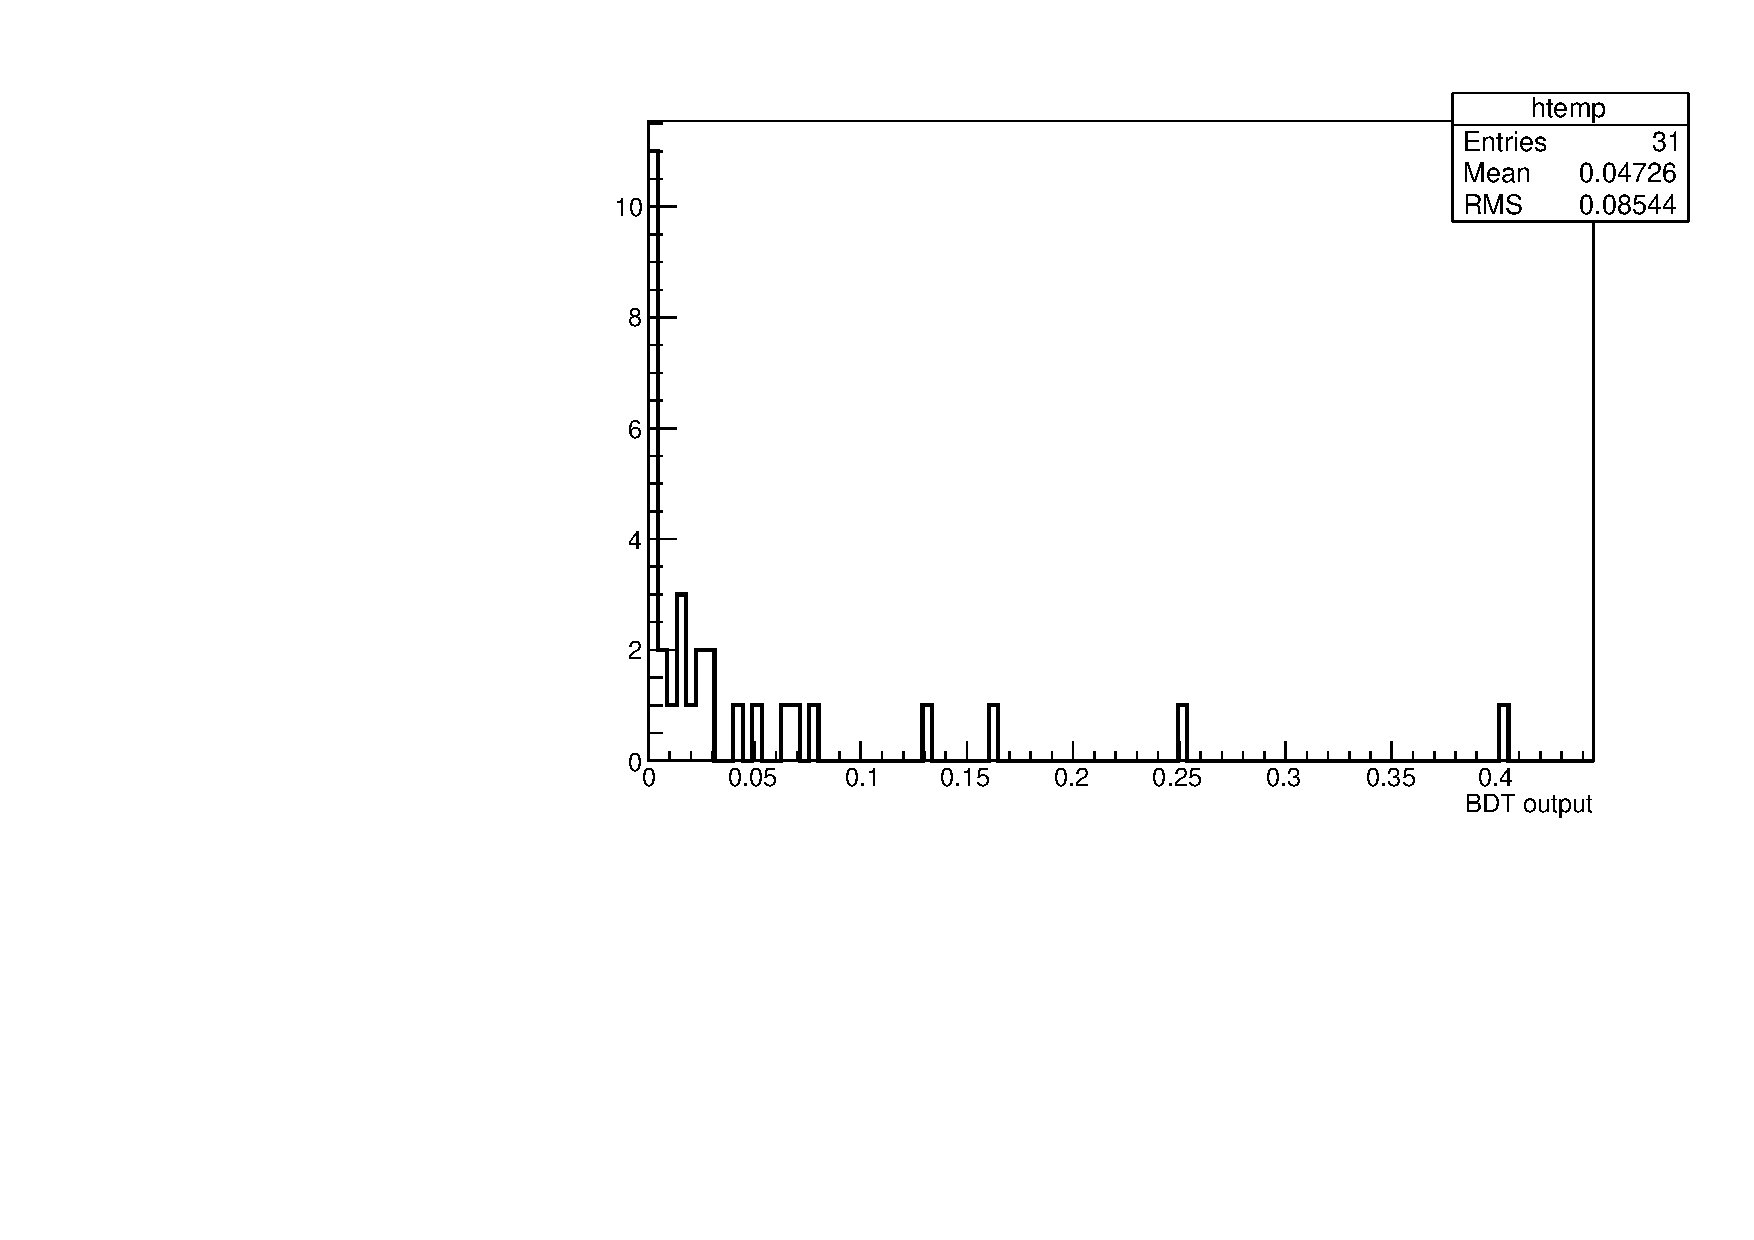
\includegraphics[scale=0.30]{figs/K3pi_BDT.pdf}
\caption{Fit to the dataset FULL including a Landau component for \KLTpi. The size of the Landau component is consistent with zero at one sigma in all BDT bins. \label{fig:fitK3pi}}
\end{center}
\end{figure}


\begin{figure} [htb!]
\begin{center}
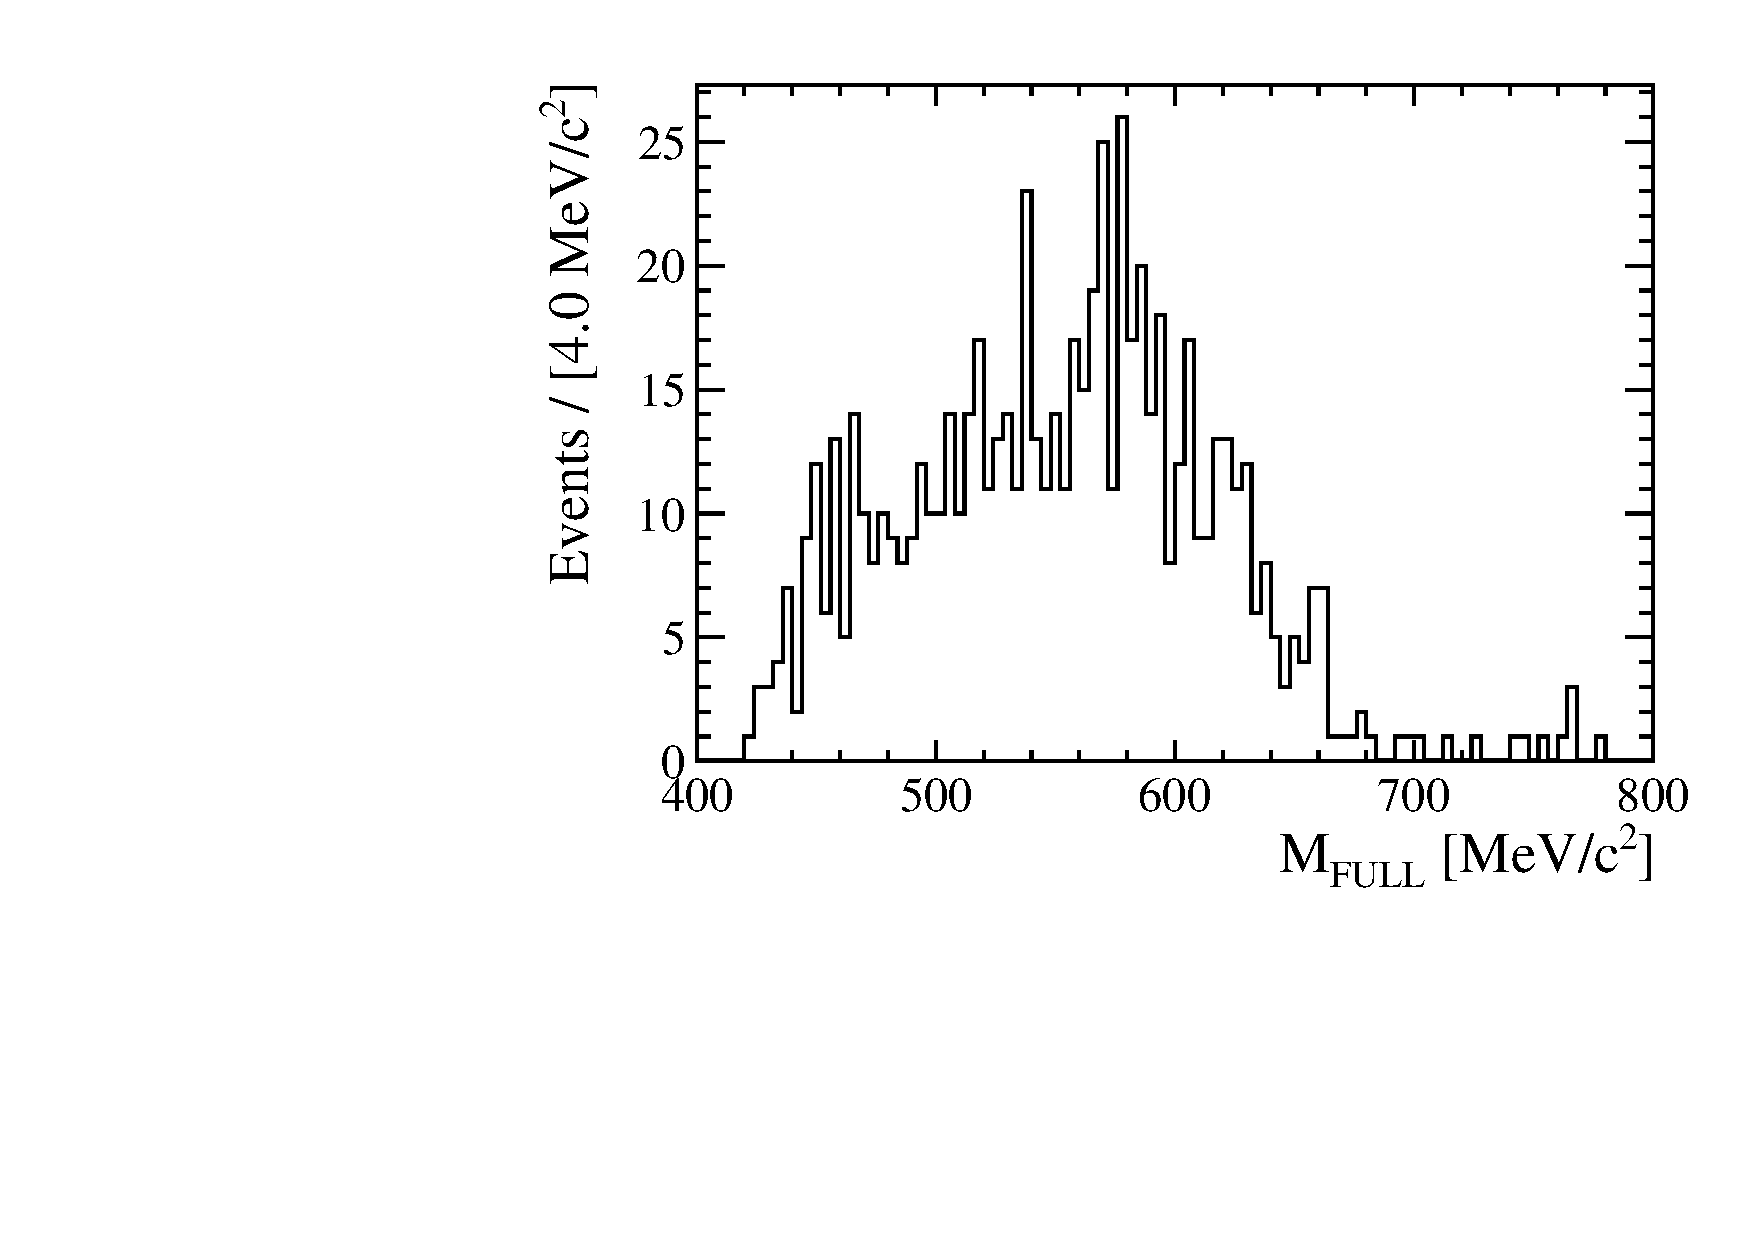
\includegraphics[scale=0.30]{figs/M_VC_pipi_hyp.pdf}
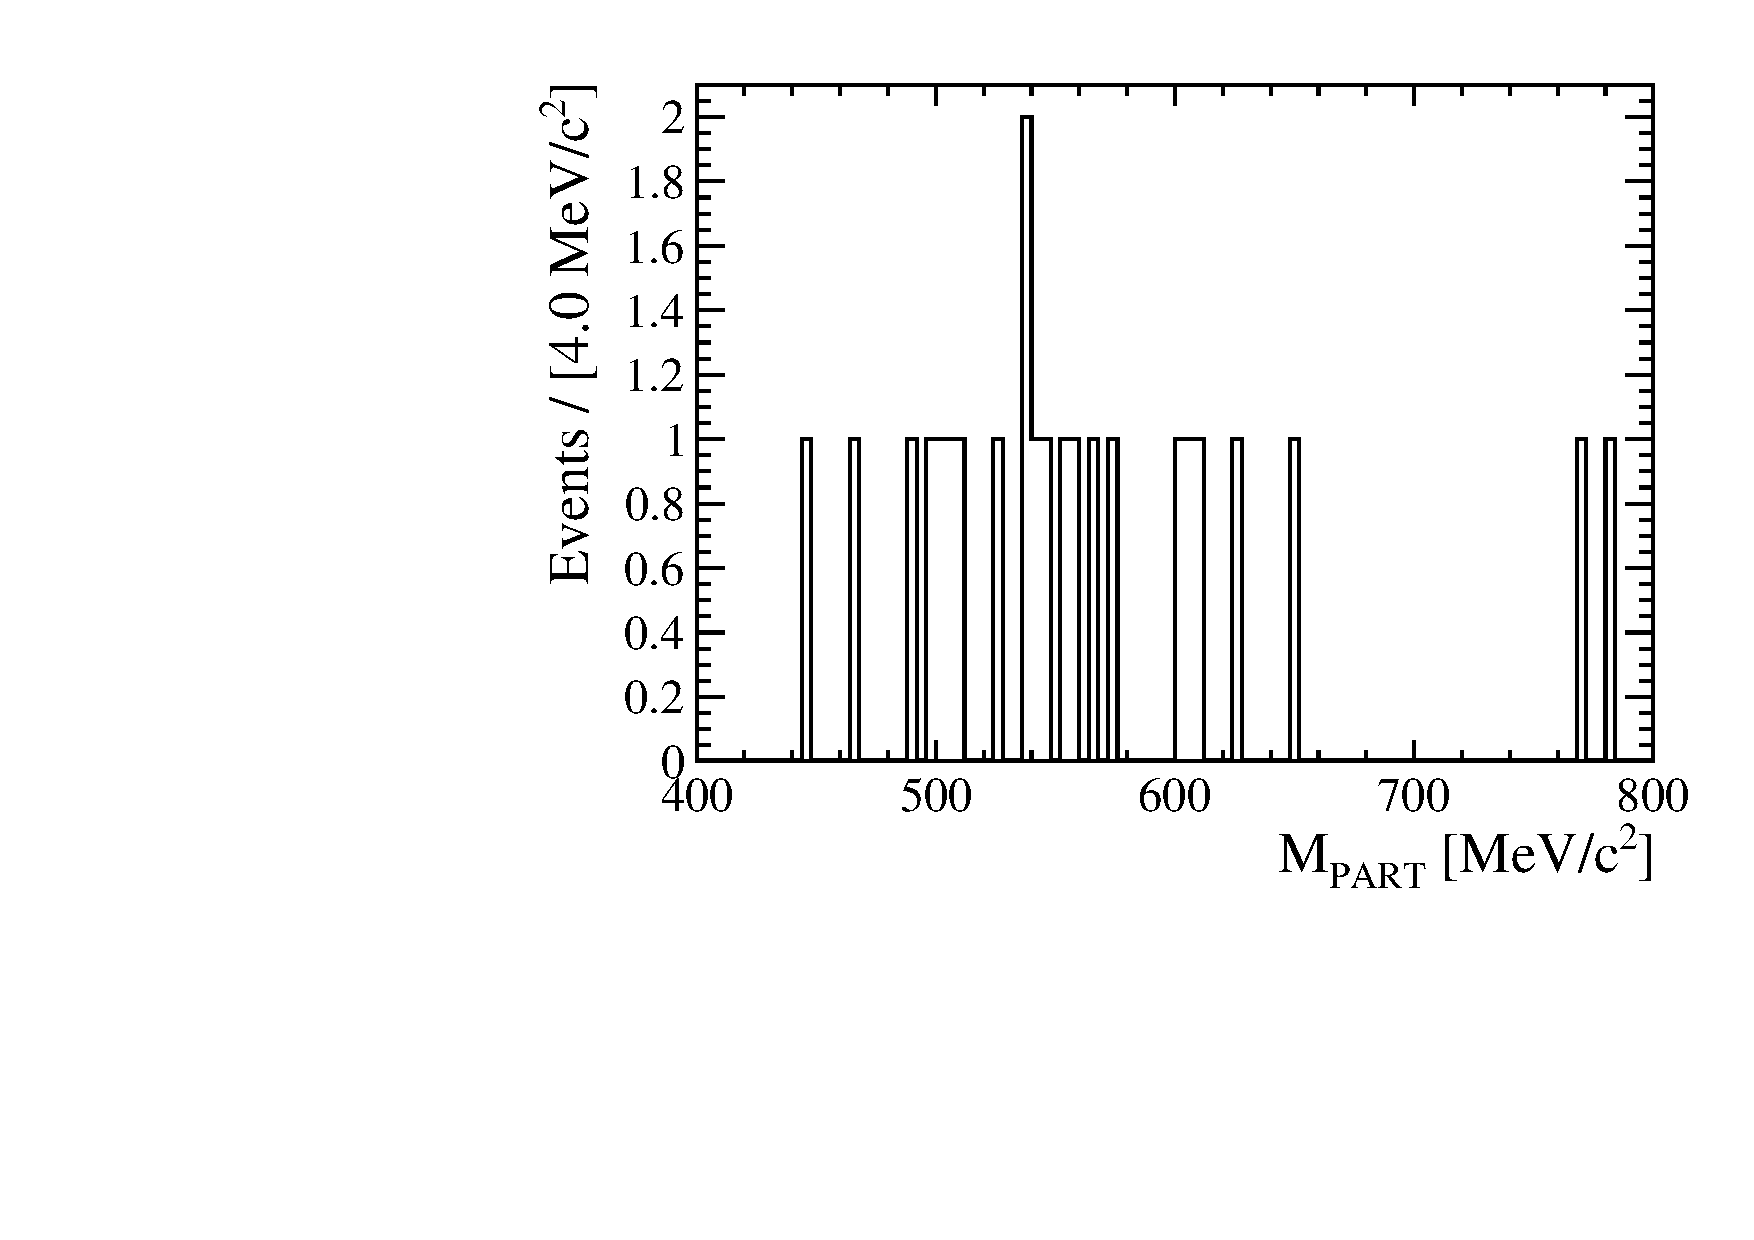
\includegraphics[scale=0.30]{figs/M_V0_pipi_hyp.pdf}
\caption{Invariant $\pi^{+}\pi^{-}\pi^0$ mass distribution of kaon candidates in decays in the FULL (left) and PARTIAL (right) data samples. The kaon mass is reconstructed using the pion mass hypothesis for the muons. \label{fig:eta_bkg}}
\end{center}
\end{figure}


